

% Gradient Info
  
\tikzset {_26yuz05ol/.code = {\pgfsetadditionalshadetransform{ \pgftransformshift{\pgfpoint{0 bp } { 0 bp }  }  \pgftransformrotate{0 }  \pgftransformscale{2 }  }}}
\pgfdeclarehorizontalshading{_0h6tu1ewh}{150bp}{rgb(0bp)=(0.94,0.98,1);
rgb(37.5bp)=(0.94,0.98,1);
rgb(49.25bp)=(0.8,0.92,1);
rgb(62.5bp)=(0.63,0.86,1);
rgb(100bp)=(0.63,0.86,1)}

% Gradient Info
  
\tikzset {_i4cvyxn0y/.code = {\pgfsetadditionalshadetransform{ \pgftransformshift{\pgfpoint{0 bp } { 0 bp }  }  \pgftransformrotate{0 }  \pgftransformscale{2 }  }}}
\pgfdeclarehorizontalshading{_2wfq3q3ve}{150bp}{rgb(0bp)=(1,1,1);
rgb(37.5bp)=(1,1,1);
rgb(62.5bp)=(0.9,0.9,0.9);
rgb(100bp)=(0.9,0.9,0.9)}
\tikzset{every picture/.style={line width=0.75pt}} %set default line width to 0.75pt        

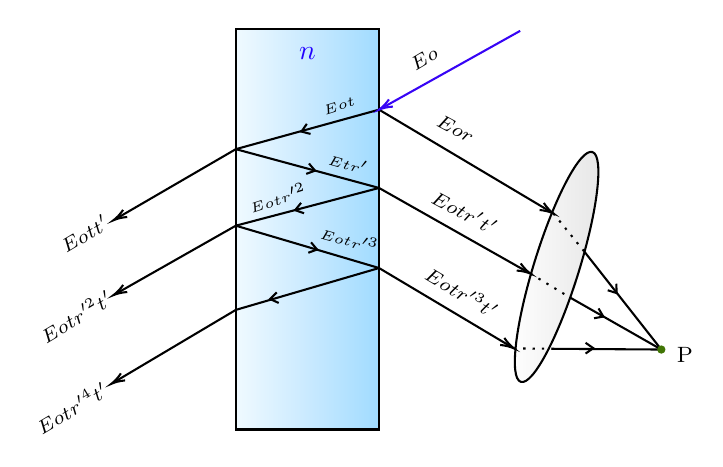
\begin{tikzpicture}[x=0.75pt,y=0.75pt,yscale=-1,xscale=1]
%uncomment if require: \path (0,300); %set diagram left start at 0, and has height of 300

%Shape: Rectangle [id:dp032628939091736475] 
\path  [shading=_0h6tu1ewh,_26yuz05ol] (163,40) -- (232,40) -- (232,233.08) -- (163,233.08) -- cycle ; % for fading 
 \draw   (163,40) -- (232,40) -- (232,233.08) -- (163,233.08) -- cycle ; % for border 

%Shape: Ellipse [id:dp7595942667517073] 
\path  [shading=_2wfq3q3ve,_i4cvyxn0y] (300.31,210.14) .. controls (294.58,208.35) and (297.65,182.12) .. (307.16,151.54) .. controls (316.68,120.96) and (329.05,97.62) .. (334.78,99.41) .. controls (340.51,101.19) and (337.45,127.43) .. (327.93,158) .. controls (318.41,188.58) and (306.05,211.92) .. (300.31,210.14) -- cycle ; % for fading 
 \draw   (300.31,210.14) .. controls (294.58,208.35) and (297.65,182.12) .. (307.16,151.54) .. controls (316.68,120.96) and (329.05,97.62) .. (334.78,99.41) .. controls (340.51,101.19) and (337.45,127.43) .. (327.93,158) .. controls (318.41,188.58) and (306.05,211.92) .. (300.31,210.14) -- cycle ; % for border 

%Straight Lines [id:da885754443074379] 
\draw    (331,147.5) -- (368,194.57) ;
%Straight Lines [id:da8784939845117902] 
\draw    (324,169.5) -- (368,194.57) ;
%Straight Lines [id:da7661126202432749] 
\draw    (315,194.2) -- (368,194.57) ;
%Straight Lines [id:da05051142310491619] 
\draw    (232,79) -- (314.28,127.98) ;
\draw [shift={(316,129)}, rotate = 210.76] [color={rgb, 255:red, 0; green, 0; blue, 0 }  ][line width=0.75]    (6.56,-1.97) .. controls (4.17,-0.84) and (1.99,-0.18) .. (0,0) .. controls (1.99,0.18) and (4.17,0.84) .. (6.56,1.97)   ;
%Straight Lines [id:da6448132052354727] 
\draw    (232,116.72) -- (303.26,157.05) ;
\draw [shift={(305,158.03)}, rotate = 209.51] [color={rgb, 255:red, 0; green, 0; blue, 0 }  ][line width=0.75]    (6.56,-1.97) .. controls (4.17,-0.84) and (1.99,-0.18) .. (0,0) .. controls (1.99,0.18) and (4.17,0.84) .. (6.56,1.97)   ;
%Straight Lines [id:da7382734603266705] 
\draw    (232,155.3) -- (295.28,193.01) ;
\draw [shift={(297,194.03)}, rotate = 210.79] [color={rgb, 255:red, 0; green, 0; blue, 0 }  ][line width=0.75]    (6.56,-1.97) .. controls (4.17,-0.84) and (1.99,-0.18) .. (0,0) .. controls (1.99,0.18) and (4.17,0.84) .. (6.56,1.97)   ;
%Straight Lines [id:da8438722714821767] 
\draw    (232,79) -- (163,98.03) ;
%Straight Lines [id:da6663758152395277] 
\draw    (232,116.72) -- (163,134.9) ;
%Straight Lines [id:da2878880139789143] 
\draw    (232,155.3) -- (163,175.47) ;
%Straight Lines [id:da679672018990835] 
\draw    (163,98.03) -- (105.73,131.3) ;
\draw [shift={(104,132.3)}, rotate = 329.85] [color={rgb, 255:red, 0; green, 0; blue, 0 }  ][line width=0.75]    (6.56,-1.97) .. controls (4.17,-0.84) and (1.99,-0.18) .. (0,0) .. controls (1.99,0.18) and (4.17,0.84) .. (6.56,1.97)   ;
%Straight Lines [id:da5885400756871793] 
\draw    (163,134.9) -- (105.74,167.4) ;
\draw [shift={(104,168.38)}, rotate = 330.42] [color={rgb, 255:red, 0; green, 0; blue, 0 }  ][line width=0.75]    (6.56,-1.97) .. controls (4.17,-0.84) and (1.99,-0.18) .. (0,0) .. controls (1.99,0.18) and (4.17,0.84) .. (6.56,1.97)   ;
%Straight Lines [id:da9028663597097684] 
\draw    (163,175.47) -- (104.72,210.08) ;
\draw [shift={(103,211.1)}, rotate = 329.29] [color={rgb, 255:red, 0; green, 0; blue, 0 }  ][line width=0.75]    (6.56,-1.97) .. controls (4.17,-0.84) and (1.99,-0.18) .. (0,0) .. controls (1.99,0.18) and (4.17,0.84) .. (6.56,1.97)   ;
%Straight Lines [id:da3067635211422284] 
\draw    (232,155.3) -- (163,134.9) ;
%Straight Lines [id:da28570828653091085] 
\draw    (232,116.72) -- (163,98.03) ;
%Straight Lines [id:da9377771078790403] 
\draw [color={rgb, 255:red, 55; green, 4; blue, 245 }  ,draw opacity=1 ]   (300,41.03) -- (233.75,78.03) ;
\draw [shift={(232,79)}, rotate = 330.82] [color={rgb, 255:red, 55; green, 4; blue, 245 }  ,draw opacity=1 ][line width=0.75]    (6.56,-1.97) .. controls (4.17,-0.84) and (1.99,-0.18) .. (0,0) .. controls (1.99,0.18) and (4.17,0.84) .. (6.56,1.97)   ;
\draw   (183.65,172.13) -- (179.54,170.24) -- (182.73,167.03) ;
\draw   (195.86,128.9) -- (191.58,127.42) -- (194.43,123.91) ;
\draw   (199,90.7) -- (194.63,89.55) -- (197.2,85.84) ;
\draw   (199.24,142.93) -- (202.15,146.39) -- (197.91,147.94) ;
\draw   (198.24,104.93) -- (201.15,108.39) -- (196.91,109.94) ;
\draw   (346.3,162.87) -- (346.49,167.38) -- (342.18,166.01) ;
\draw   (337.76,174.78) -- (340.05,178.68) -- (335.6,179.49) ;
%Straight Lines [id:da2986310493998955] 
\draw  [dash pattern={on 0.84pt off 2.51pt}]  (316,129) -- (331,147.5) ;
%Straight Lines [id:da6700491570854924] 
\draw  [dash pattern={on 0.84pt off 2.51pt}]  (305,158.03) -- (324,169.5) ;
%Straight Lines [id:da922121143131131] 
\draw  [dash pattern={on 0.84pt off 2.51pt}]  (297,194.03) -- (315,194.2) ;
\draw   (331.51,191.32) -- (335.22,193.91) -- (331.51,196.5) ;
%Shape: Circle [id:dp01647618202213541] 
\draw  [draw opacity=0][fill={rgb, 255:red, 65; green, 117; blue, 5 }  ,fill opacity=1 ] (366,194.57) .. controls (366,193.46) and (366.9,192.57) .. (368,192.57) .. controls (369.1,192.57) and (370,193.46) .. (370,194.57) .. controls (370,195.67) and (369.1,196.57) .. (368,196.57) .. controls (366.9,196.57) and (366,195.67) .. (366,194.57) -- cycle ;

% Text Node
\draw (192,47.4) node [anchor=north west][inner sep=0.75pt]  [color={rgb, 255:red, 34; green, 1; blue, 255 }  ,opacity=1 ]  {$n$};
% Text Node
\draw (202.74,76.34) node [anchor=north west][inner sep=0.75pt]  [font=\tiny,rotate=-342.63]  {$E\tund{o} t$};
% Text Node
\draw (207.85,97.22) node [anchor=north west][inner sep=0.75pt]  [font=\tiny,rotate=-15.79]  {$E\tund tr'$};
% Text Node
\draw (166.71,121.46) node [anchor=north west][inner sep=0.75pt]  [font=\tiny,rotate=-342]  {$E\tund{o} tr^{\prime 2}$};
% Text Node
\draw (204.08,132.38) node [anchor=north west][inner sep=0.75pt]  [font=\tiny,rotate=-15.8]  {$E\tund{o} tr^{\prime 3}$};
% Text Node
\draw (244.21,54.39) node [anchor=north west][inner sep=0.75pt]  [font=\scriptsize,rotate=-329.1]  {$E\tund{o}$};
% Text Node
\draw (261.51,78.89) node [anchor=north west][inner sep=0.75pt]  [font=\scriptsize,rotate=-28.22]  {$E\tund{o} r$};
% Text Node
\draw (259.51,114.89) node [anchor=north west][inner sep=0.75pt]  [font=\scriptsize,rotate=-28.22]  {$E\tund{o} tr't'$};
% Text Node
\draw (257.12,151.34) node [anchor=north west][inner sep=0.75pt]  [font=\scriptsize,rotate=-30.91]  {$E\tund{o} tr^{\prime 3} t'$};
% Text Node
\draw (75.21,141.39) node [anchor=north west][inner sep=0.75pt]  [font=\scriptsize,rotate=-329.1]  {$E\tund{o} tt'$};
% Text Node
\draw (65.21,184.39) node [anchor=north west][inner sep=0.75pt]  [font=\scriptsize,rotate=-329.1]  {$E\tund{o} tr^{\prime 2} t'$};
% Text Node
\draw (63.21,228.39) node [anchor=north west][inner sep=0.75pt]  [font=\scriptsize,rotate=-329.1]  {$E\tund{o} tr^{\prime 4} t'$};
% Text Node
\draw (374,192.18) node [anchor=north west][inner sep=0.75pt]  [font=\footnotesize] [align=left] {P};


\end{tikzpicture}
